\section*{Prologue}

Deep learning optimizers are often motivated from the perspectives of convex and approximate second-order theory. These theoretical frameworks have been used to inspire algorithmic ideas, as well as providing means to analyse the convergence of various optimizers. However, we believe---and will attempt to demonstrate---that there is a wealth of untapped algorithmic opportunity in the simpler realm of exact first-order theory without convexity assumptions.


To make our case, we choose three optimizers that were originally analysed under convex or approximate second-order theory: Adam, Shampoo and Prodigy. After disabling their exponential moving averages (EMA), we show that each algorithm admits a parsimonious theoretical explanation as a variant of \textit{steepest descent} under a certain norm. EMA can then be thought of as ``smoothing out'' the algorithm, or making it more robust to mini-batch noise, although nailing down the precise role of EMA is perhaps still an open problem.

By steepest descent, we mean the procedure of choosing a weight update $\Delta \vw$ to minimise a local quadratic model of the loss function $\el$ of the form $\el(\vw) + \nabla_\vw \el(\vw)^\top\Delta\vw + \frac{\lambda}{2}\cdot \norm{\Delta \vw}^2$, visualized in \cref{fig:contours}. Crucially, the \textit{sharpness parameter} $\lambda$ and \textit{norm} $\norm{\cdot}$ are chosen a priori, without touching an (approximate) Hessian during training. As such, we consider steepest descent to be a squarely first-order method and not an (approximate) second-order method.

Throughout the anthology, we rely on a dual description of steepest descent:
\begin{myproposition}[Steepest descent]\label{prop:steepest} For any $\vg \in \R^n$ thought of as ``the gradient'' and any $\lambda \geq 0$ thought of as ``the sharpness'', and for any norm $\norm{\cdot}:\R^n\to\R$ with dual norm $\norm{\cdot}^\dagger$:
\begin{align}\label{eq:dual-steepest}
    \argmin_{\Delta \vw \in \R^n} \left[\vg^\top \Delta \vw + \frac{\lambda}{2} \, \norm{\Delta \vw}^2 \right] = - \frac{\norm{\vg}^\dagger}{\lambda} \cdot \argmax_{\norm{\vt}=1} \vg^\top \vt.
\end{align}
\end{myproposition}
\cref{eq:dual-steepest} separates the solution of the steepest descent problem into two pieces: first computing the \textit{step size} as the dual norm of the gradient divided by the sharpness, and second solving for the \textit{step direction} as the unit vector that maximizes the inner product with the gradient. The proof of this proposition is given in \cref{proof:steepest}.

\begin{figure}
    \centering
    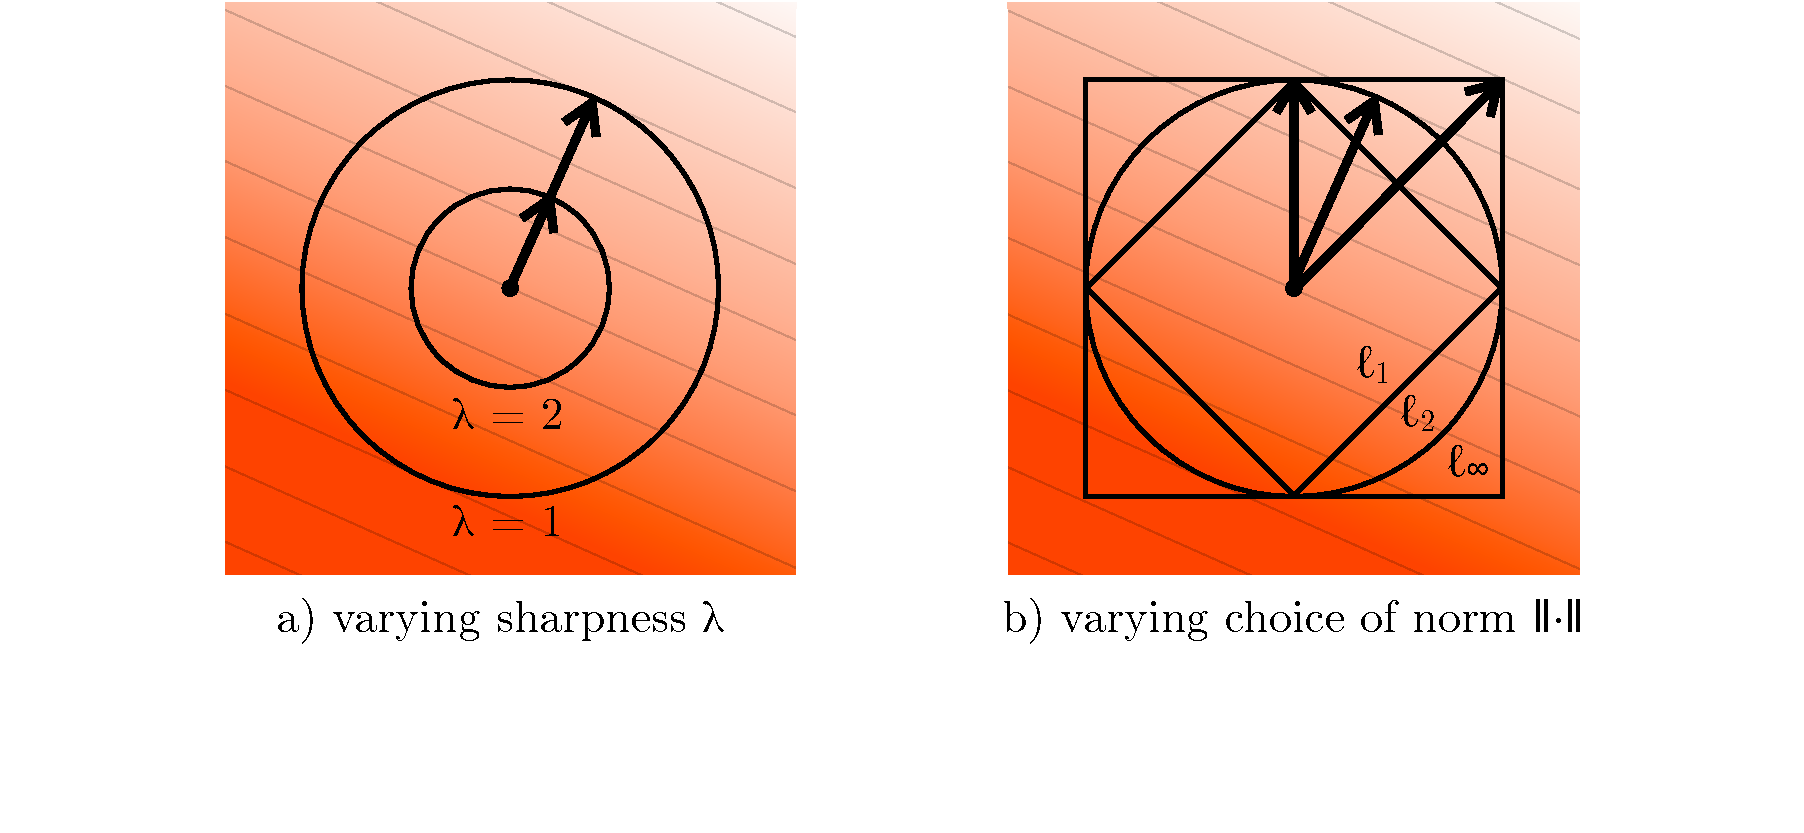
\includegraphics[width=\linewidth,trim={0 3.2cm 0 0},clip]{figure/norms}
    \vspace{-1em}
    \caption{Steepest descent considers the problem of minimizing a linear functional under a quadratic penalty: $\argmin_{\Delta \vw \in \R^n} \left[\vg^\top \Delta \vw + \frac{\lambda}{2} \, \norm{\Delta \vw}^2 \right]$ for $\vg \in \R^n$. Here we show how the solution varies with the sharpness $\lambda > 0$ and the choice of norm $\norm{\cdot}$. We overlay different norm balls on top of a linear color gradient, and use arrows to denote the solution, meaning the member of the norm ball that ``minimizes the color''. a) Increasing the sharpness decreases the size of the solution vector. b) Changing the norm can change the direction of the solution vector. For different $\ell_p$ norms, the solution direction changes because the gradient is not axis-aligned. In practice, we should pick the sharpness and norm to fit the geometry of our loss.}
    \label{fig:contours}
\end{figure}


Of course, the art of steepest descent lies in choosing a norm $\norm{\cdot}$ and a sharpness $\lambda$ suited to the optimization problem at hand. While it may be possible to turn this art into a science \citep{modula}, that ambition is beyond the scope of this anthology. Here we point out that past methods do implicitly make decisions about norms, and in a somewhat haphazard manner. In fact, they implicitly assign different \textit{induced matrix norms} to the network layers:

\begin{mydefinition}[Induced 
operator norm]\label{def:induced} Given a matrix $\mM\in\R^{d_\out \times d_\inn}$ and two normed vector spaces $(\R^{d_\inn},\norm{\cdot}_\alpha)$ and $(\R^{d_\out},\norm{\cdot}_\beta)$, the ``$\alpha$ to $\beta$'' induced operator norm is given by:
\begin{equation}
    \norm{\mM}_{\alpha\to\beta} = \max_{\substack{\vx \in \R^{d_\inn}}} 
    \frac{\norm{\mM\vx}_\beta}{\norm{\vx}_\alpha}.
\end{equation}
\end{mydefinition}
\cref{def:induced} tells us that by varying the choice of vector norms $\norm{\cdot}_\alpha$ and $\norm{\cdot}_\beta$, we can induce a large family of matrix norms. In turn, this implies a correspondingly large family of steepest descent optimizers. By foregrounding this issue, we hope that algorithm designers may develop more suitable optimizers by becoming more intentional about their choice of norm.
